\chapter{TESTING AND RESULTS}
\label{ch:testing}

Basic message transfer from Author to Recipients is accomplished by using an asynchronous store-and-forward communication infrastructure in a sequence of independent transmissions through some number of mail transfer agents\cite{rfc5598}. Two of the most common ways to analyze the architecture was to consider the time required to send all the emails and the cost associated with it. Both of the metrics are analysed in the following section.

\section{Performance}
There are two performance monitoring services available to AWS application developers: CloudWatch and X-ray.\cite{lin2018tracking}
 The application is analyzed to see the time required to send the emails and the time taken to run the functions between the request and response to the API endpoint. This can be seen through the cloudwatch\cite{awscloudwatch} logs and X-ray to find out the issues with latency over various regions and finding the best regions and how to optimize the functions.In this case, we used X-Ray as a monitoring and display service that automatically samples the entry and exit of function instances, called segments, using unique trace identifiers \textbf{\texttt{(trace\_id)}}\cite{lin2018tracking}\cite{awsxray}.\par

 Here we take the case of sending multiple emails and the time taken is sampled over 30 data points to represent in Figure 2. The time is calculated by considering the cloudwatch logs that can be used to determine the time taken to execute the last function of lambda as show in Figure 1 to send the email and the time leading to that function from the start of the API gateway request log that is stored in the logs. This experimented several times to cancel out the variations of cold start that is a common phenomenon in serverless functions. All the calculations are done to avoid any overlap between different invocations and only a single request is sent within the same region.\par

\begin{figure}[H]

	\centering
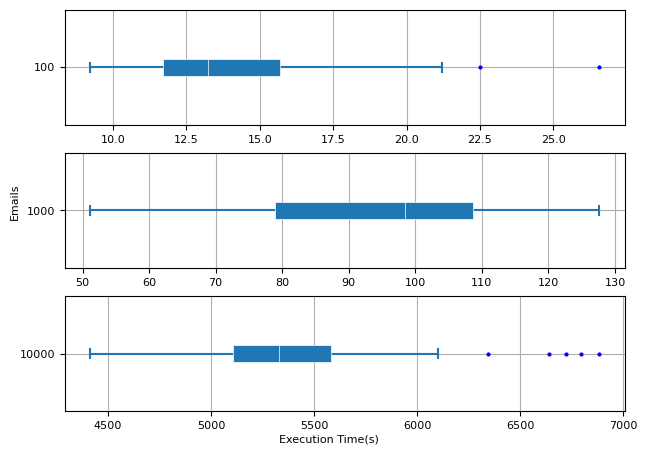
\includegraphics[width=\textwidth]{figures/general_analysis.png}
	\caption{Boxplot depicting the distrubtion of backend runtimes.}
	\label{fig:general}
\end{figure}
In Figure \ref{fig:general} the graph depicts boxplot of runtimes of serverless backend functions after the api is invoked and when email is sent, the number of emails sent is directly proportional to the time taken. The time taken for 10,00 emails averaging at around 30 minutes is sufficient and satisfactory considering that the time taken is to derived from the last email that is sent in the list of emails.  
\section{Error Handling}

Errors in the frontend of the web application is managed by notification pop-up windows that can signify corrections of problems in execution that have occurred.

	

\begin{figure}[H]
\centering
\begin{minipage}[c]{.5\textwidth}
  \centering
  
\includegraphics[width=.9\linewidth]{figures/frontend_error_1.png}
\end{minipage}\hfill
\begin{minipage}[c]{.5\textwidth}
  \centering
  
\includegraphics[width=.9\linewidth]{figures/frontend_errors_2.png}
\end{minipage}\\
\vspace{0.3cm}

\begin{minipage}[c]{.5\textwidth}
  \centering
  
\includegraphics[width=.9\linewidth]{figures/frontend_errors_3.png}
\end{minipage}%
\begin{minipage}[c]{.5\textwidth}
  \centering
  
\includegraphics[width=.9\linewidth]{figures/frontend_errors_4.png}
\end{minipage}\\
\caption{Different Error Messages}
\label{fig:different-errors}
\end{figure}

As shown in Figure \ref{fig:different-errors} If the user leaves out important information that is required by the API. The application halts giving meaningful error messages in a pop-up box at the right corner of screen. 

\section{Cost}
The cost of the services can also be a motivating factor to implement such an architecture. In our use case The following architecture can be tested with the AWS free tier and later expanded to the needs of the users. With \$0.01 dollars per 1,000 emails but one needs to be wary about the associated services like the SES, SNS and the cloudwatch metrics to analyze the emails add up to cost but since they are calculated based on the GB of data it needs to pre-process the rates will not exceed the cost of emails.

Here we take the example, provided by the SES platform to estimate the cost required to implement the architecture.

You use Amazon SES to send about 250,000 emails per month. You receive 1,000 emails per month. You don't use dedicated IP addresses. Every message you send and receive is 32KB in size which results in a total of \$25.98 per month \cite{sespricing} which is significantly less than competitors such as SendGrid or MailChimp who offer their own SMTP server or schedule emails to fit into the constraints of other providers to carry out email campaigns. \par



Amazon provides sample pricing calculations,but as your workload varies, so will the billing. \cite{eivy2017wary} The SQS requests can exceed the free tier if not monitored carefully and add up to additional costs for the next 1000 requests or more based on the usage of the system.\par


\newpage


\section{Results}

The bulk email application has successfully achieved its objective of sending emails in large volumes using the web interface that is provided passing all the test cases and error handling mechanisms. The customization that is proposed is also accomplished by the SES template.

\begin{table}[H]
    \centering
    \begin{tabularx}{.7\textwidth}{| X | X | X | X | X |}
    %\begin{tabularx}{\textwidth}{sssss}
        \hline
        Serial \hspace{0.2cm} Number      & Number of emails     & Mean time taken in (ms) & Median time taken in (ms)\\ \hline
        1         & 100      	  & 14.5        & 13.2     \\ \hline
        2         & 1,000         & 93.4        & 98.4   \\ \hline
        3         & 10,000        & 5511.5       & 5329.9   \\ \hline
    \end{tabularx}
    \caption{Time taken for different volumes of emails}
	    \label{table:time}
\end{table}

In Table \ref{table:time} The time taken by different volumes of email such as 100,1000,1000 taken from the box plot in Figure \ref{fig:general} is used.

\subsection{Dashboard}

The analysis of metrics that are obtained from the sending of emails can be viewed in the form of a high level dashboard and can be shared for real time monitoring of the bounce rate and minimise it and track the success of the email campaign for a specific sending email address.

\begin{figure}[H]
            \centering
            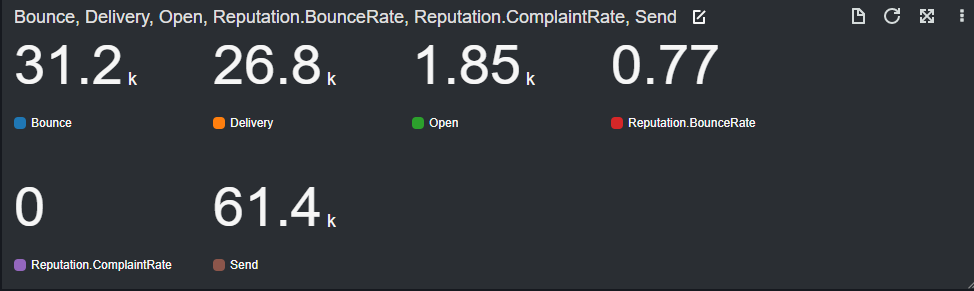
\includegraphics[width=160mm]{figures/dashboard.png}
            \caption{Statistics Dashboard of email services}
	    \label{fig:dashboard}
\end{figure}


As shown the Figure \ref{fig:dashboard}, The various mertrics such as open,sent,delivered,bounced are obtained and are updated in real time with a specific time interval. The duration and time can be changed using filtering options to analyse the campaigns effectively.
